% !TEX root = ../main.tex
%
\chapter{Experiments}
\label{sec:experiments}
To validate the effectiveness of our proposed Credal Semantic
Entropy method, we conducted a series of experiments on a 
standard free-form Question Answering (QA) benchmark.
The primary objective of these experiments is to evaluate
whether quantifying epistemic uncertainty via valid 
temperatures provides a more reliable signal for high uncertainty 
than standard single-point metrics.


\section{Experimental Setup}
\label{sec:experiments:setup}

\subsection{Dataset: CoQA}
\label{sec:experiments:setup:coqa}
We utilized the \textbf{Conversational Question Answering (CoQA)} 
dataset \parencite{reddy2019coqaconversationalquestionanswering}
for our evaluation. CoQA is a large-scale dataset for building
Conversational Question Answering systems. It contains 127k+ 
questions with answers obtained from 8k+ conversations about 
text passages from seven diverse domains 
\parencite{reddy2019coqaconversationalquestionanswering}.

For our specific task, we followed the 
experimental protocol established by 
\textcite{kuhn2023semanticuncertaintylinguisticinvariances}.
We used the development split of CoQA, which provides a diverse 
set of questions. The dataset was split into a \textbf{calibration set} 
(used to determine the valid temperature set) and a \textbf{test set}
(used to evaluate the final uncertainty metrics).


\subsection{Model Architecture}
\label{sec:experiments:setup:model}
All experiments were conducted using the \textbf{Opt-6.7B} model
\parencite{zhang2022opt}. OPT (Open Pre-trained Transformer) is a 
decoder-only architecture that replicates the performance and 
behaviour of GPT-3 \parencite{brown2020languagemodelsfewshotlearners}.
We chose the 6.7B parameter variant as it strikes a balance between
computational feasibility and the capability to generate coherent text.

For the semantic clustering step, we employed a \textbf{DeBERTa-large-MNLI}
model \parencite{he2021debertadecodingenhancedbertdisentangled} to assess
bidirectional entailment between generated answers.

\subsection{Baselines}
\label{sec:experiments:setup:baselines}
We compared our proposed \textbf{Credal Semantic Entropy (Credal SE)}
against several strong baselines:

\begin{itemize}
	\item \textbf{Semantic Entropy (SE)}: The original
	    metric proposed by 
	    \textcite{kuhn2023semanticuncertaintylinguisticinvariances},

	\item \textbf{Lexical Similarity (ROUGE-L)}: We compute the average
	    ROUGE-L score across all pairs of the $N$ sampled sequences.
	    Lower average similarity indicates higher lexical dispersion
	    (uncertainty).
	    \parencite{lin-2004-rouge}.

	\item \textbf{Predictive Entropy (PE)}: The standard entropy of the 
	    model's output distribution over the sequence of tokens.
	    Unlike semantic entropy, this metric considers every lexical 
	    variation as a distinct outcome, calculating uncertainty
	    directly on the raw strings without semantic clustering
	    \parencite{malinin2021uncertaintyestimationautoregressivestructured}.

	\item \textbf{Length-Normalized PE}: A variant of Predictive Entropy
	    that normalizes the sum of token entropies by the sequence 
	    length, mitigating the bias against longer answers
	    \parencite{malinin2021uncertaintyestimationautoregressivestructured}.

	\item \textbf{Margin Measure (MM)}: The difference in
	    log-probability between the most likely sequence and the second
	    most likely sequence. A small margin indicates high uncertainty
	    between the top two choices \parencite{lin-etal-2022-towards}.

	\item \textbf{P(true)}: A self-evaluation metric 
	    \parencite{kadavath2022languagemodelsmostlyknow} 
	    where the model is prompted with the question and its generated
	    answer, and asked to output ``True'' or ``False''. We extract the
	    probability mass assigned to the ``True'' token.
\end{itemize}

\subsection{Evaluation Metric: AUROC}
\label{sec:experiments:setup:evaluation}
To quantify the performance of each uncertainty method, we treat
uncertainty quantification as a binary classification problem. The core
task is to determine if the uncertainty score can reliably distinguish
between correct and incorrect model generations. We use the answers
that were generated by the model using the temperature with the 
maximum likelihood.

\textbf{Ground Truth Labeling} \\
To establish the ground-truth labels for our experiments, we compare 
the generated answers against the gold-standard reference answer 
provided in the CoQA dataset. We define correctness based on lexical 
overlap using the \textbf{ROUGE} metric (Recall-Oriented Understudy 
for Gisting Evaluation) 
\parencite{lin-2004-rouge}. Specifically, a generated answer is 
labeled as:

\begin{itemize}
	\item \textbf{Correct}: If the ROUGE-L score between the 
	    generation and the reference is strictly greater than $0.3$.

	\item \textbf{Incorrect}: If the ROUGE-L score is less than or 
	    equal to $0.3$.
\end{itemize}

This threshold allows for minor phrasing differences while ensuring
that the core semantic content overlaps significantly with the reference.

\textbf{AUROC Calculation} \\
We report the 
\textbf{Area Under the Receiver Operating Characteristic curve (AUROC)}
\parencite{BRADLEY19971145}.
The AUROC represents the probability that a randomly selected incorrect 
answer will have a higher uncertainty score than a randomly 
selected correct answer.

\begin{itemize}
    \item $\text{AUROC} = 0.5$: Indicates random performance 
	(no better than a coin flip)

    \item $\text{AUROC} = 1.0$: Indicates perfect detection 
	(all incorrect answers have higher uncertainty scores than all 
	correct answers).
\end{itemize}

\section{Results}
\label{sec:experiments:results}
As discussed in the methodology, constructing a credal set via 
multi-temperature-sampling incurs significant computational overhead.
To maintain a feasible evaluation pipeline while ensuring sufficient
granularity, we restricted our analysis to the temperature interval
$[0.4, 2.2]$ evaluated at two distinct resolutions:  
a 20-step grid (Table \ref{tab:twenty_steps_interval}) and a 
50-step grid (Table \ref{tab:fifty_steps_interval}).

Our evaluation is conducted on a subset of approximately 2400 queries, using
60\% ($\approx 1440$ questions) of the questions to find valid
temperatures and the other 40\% ($\approx 960$ questions) to evaluate our 
uncertainty estimation, from the CoQA development set.
In this section, we systematically present the
uncertainty quantification performance (measured using AUROC) across
these configurations, exploring how the grid resolution and the relative
likelihood threshold $\alpha$ impact the robustness of our uncertainty
estimates.


\subsection{Evaluation: 20-Step Interval}
\label{sec:experiments:results:twenty_steps_interval}
We begin our analysis using the coarser 20-step temperature interval 
combined with a highly restrictive relative likelihood threshold of 
$\alpha=0.9$. Table \ref{tab:results_20_steps_alpha07} summarizes
the AUROC scores for our proposed Credal Semantic Entropy alongside 
the established single-point baselines. The baselines were evaluated on
the generations predicted by the model using the most likely temperature 
($\tau = 1.347$).

Table \ref{tab:results_20_steps_alpha07}: 
	Hallucination detection performance (AUROC) on the CoQA subset
	using a 20-step temperature interval and a strict relative
	likelihood threshold ($\alpha=0.9$). Metrics compared are our
	proposed Credal Semantic Entropy (Credal SE), standard Semantic
	Entropy (SE), Predictive Entropy (PE), length-normalized Predictive
	Entropy (ln PE), Margin Measure (MM), P(true) and
	Lexical Similarity (LS).
\begin{table}[h]
    \centering
    \begin{tabular}{lccccccc}
        \toprule
	\textbf{Configuration} & \textbf{Credal SE} & \textbf{SE} & \textbf{PE} & \textbf{ln PE} & \textbf{MM} & \textbf{P(true)} &\textbf{LS}\\
        \midrule
    20 Steps, $\alpha = 0.7$ & 0.60 & 0.61 & 0.58 & 0.66 & 0.57 & 0.59 		&\textbf{0.70}\\
        \bottomrule
    \end{tabular}
    \caption{}
    \label{tab:results_20_steps_alpha07}
\end{table}

\begin{figure}
    \center
    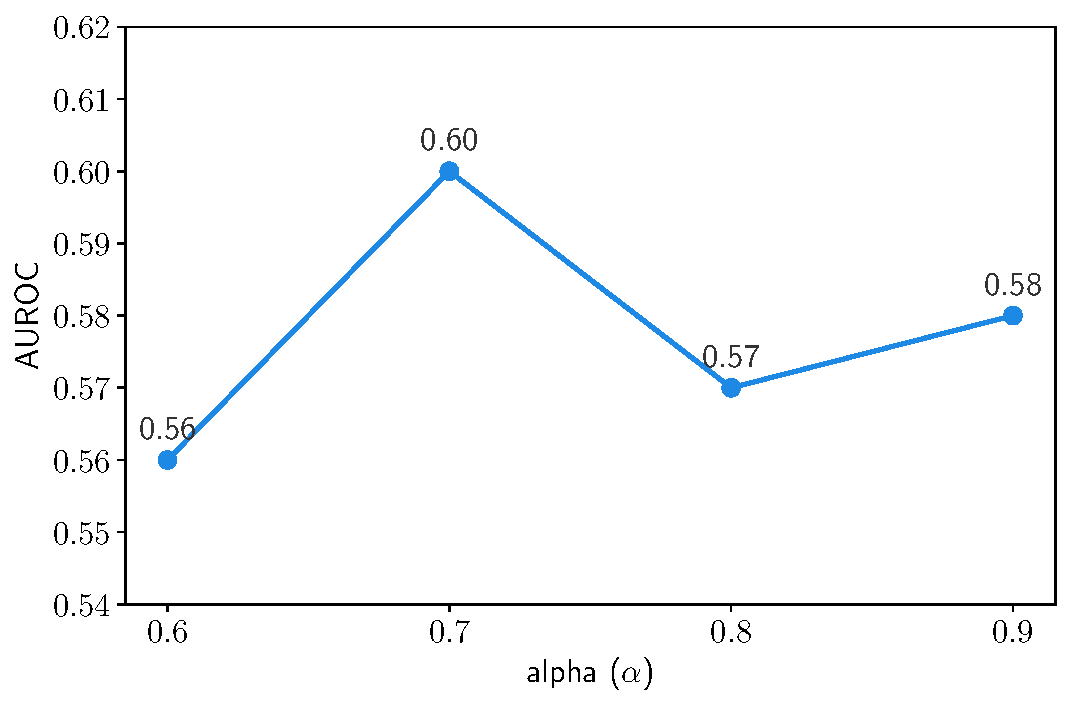
\includegraphics[width=0.6\textwidth]{gfx/alpha_results_lineplot_20_steps.pdf}
    \caption{Impact of the relative likelihood threshold ($\alpha$) on
    the uncertainty quantification performance of 
    Credal Semantic Entropy.
    The line plot illustrates the AUROC scores evaluated on the 20-step
    temperature grid for $\alpha \in \{0.6, 0.7, 0.8, 0.9\}$.}
    \label{fig:experiments:aurocs_alphas_20_steps}
\end{figure}

\textbf{Analysis of 20-Step Results} \\
Under this specific configuration, Lexical Similarity (LS) achieves the
strongest performance with an AUROC of 0.70, followed by length-normalized
Predictive Entropy (ln PE) with 0.66.
Our proposed Credal Semantic Entropy yields an AUROC of 0.58, which
underperforms standard Semantic Entropy (0.61) and equals raw Predictive 
Entropy (0.58).


\subsection{Evaluation: 50-Step Interval}
\label{sec:experiments:results:fifty_steps_interval}
To investigate whether a finer resolution of the temperature space 
improves the calibration of our credal set, we extend our analysis to the
50-step interval (Table \ref{tab:fifty_steps_interval}). As in the previous
experiment, we first evaluate the most restrictive threshold, $\alpha=0.9$.

Table \ref{tab:results_50_steps_alpha09}:
	Hallucination detection performance (AUROC) on the CoQA subset
	using a 50-step temperature interval and a strict relative
	likelihood threshold ($\alpha=0.9$). Metrics compared are our
	proposed Credal Semantic Entropy (Credal SE), standard Semantic
	Entropy (SE), Predictive Entropy (PE), length-normalized Predictive
	Entropy (ln PE), Margin Measure (MM), P(true) and
	Lexical Similarity (LS).
\begin{table}[h]
    \centering
    \begin{tabular}{lccccccc}
        \toprule
	\textbf{Configuration} & \textbf{Credal SE} & \textbf{SE} & \textbf{PE} & \textbf{ln PE} & \textbf{MM} & \textbf{P(true)}
			    &\textbf{LS}\\
        \midrule
	50 Steps, $\alpha = 0.9$ &0.56 &0.62 &0.55 &0.65 &0.54 &0.62
			    &\textbf{0.68}\\
        \bottomrule
    \end{tabular}
    \caption{}
    \label{tab:results_50_steps_alpha09}
\end{table}

\textbf{Analysis of 50-Step Results} \\
Table \ref{tab:results_50_steps_alpha09} demonstrates that under the 50-step
configuration at $\alpha=0.9$, lexical similarity (LS)
maintains its position as the strongest baseline with an AUROC of o.68,
again followed by length-normalized Predictive Entropy (ln PE).
Standard Semantic Entropy (SE) and P(true) perform competitively at 0.62.

Crucially, our proposed Credal Semantic Entropy yields an AUROC of 0.56. 
Notably, this is a slight degradation compared to its performance on the 
coarser 20-step grid (0.58).
Note that we were not able to test more 
$\alpha$ values for the 50-step interval as it was
computationally prohibitive.


\subsection{Additional Evaluation: Local Analysis at $\tau=0.5$}
\label{sec:experiments:results:additional}
In our primary evaluations, the single-point baselines were evaluated at
$\tau \approx 1.39$, as this was the temperature that maximized the average 
likelihood of the calibration data ($\tau^{ML}$). However, 
\textcite{kuhn2023semanticuncertaintylinguisticinvariances} reported that
standard semantic entropy achieves peak performance at a significantly lower
temperature, specifically $\tau=0.5$.
To ensure a fair and comprehensive comparison against this baseline, we 
conducted an additional evaluation centered around this lower temperature
regime.

\textbf{Methodological Caveat: Local Relative Likelihood} \\
Applying our framework strictly, a temperature of $\tau=0.5$ possesses a 
global relative likelihood close to zero when compared to the true optimum
at $\tau \approx 1.39$, and would thus be excluded by any reasonable 
$\alpha$-cut. Consequently, for this specific evaluation, we compute a
\textit{local} relative likelihood. We restricted our grid to a narrow
15-step interval around the baseline's optimum, specifically 
$[0.490, 0.505]$ with a step size of 0.001. Within this local grid, the
maximum likelihood was observed at $\tau=0.505$. Applying an 
$\alpha$-threshold of 0.9 yielded a valid temperature set of 
$\mathcal{T}_{0.9} = \{0.497, 0.498, \dots, 0.505\}$.

\textbf{Results} \\
Table \ref{tab:results_opt_sem_entropy}:
	Hallucination detection performance (AUROC) on the CoQA subset
	using a 15-step temperature interval and a strict relative
	likelihood threshold ($\alpha=0.9$). Metrics compared are our
	proposed Credal Semantic Entropy (Credal SE), standard Semantic
	Entropy (SE), Predictive Entropy (PE), length-normalized Predictive
	Entropy (ln PE), Margin Measure (MM), P(true) and
	Lexical Similarity (LS).
\begin{table}[h]
    \centering
    \begin{tabular}{lccccccc}
        \toprule
	\textbf{Configuration} & \textbf{Credal SE} & \textbf{SE} & \textbf{PE} & \textbf{ln PE} & \textbf{MM} & \textbf{P(true)} &\textbf{LS}\\
        \midrule
    15 Steps, $\alpha = 0.9$ & 0.67 & \textbf{0.74} & 0.64 & 0.72 & 0.61 & 0.69 &0.61\\
        \bottomrule
    \end{tabular}
    \caption{}
    \label{tab:results_opt_sem_entropy}
\end{table}

Under this configuration, Semantic Entropy (SE) achieves the 
highest overall AUROC of 0.74, closely followed by 
length-normalized Predictive Entropy (0.72). Our proposed Credal Semantic
Entropy achieves a score of 0.67, outperforming raw Predictive Entropy 
(0.64) and Lexical Similarity (0.61), but falling short of the leading 
baselines.

\section{Discussion}
\label{sec:experiments:discussion}
The empirical evaluation of Credal Semantic Entropy
presents a nuanced picture of uncertainty quantification
in LLMs. While the credal framework offers a mathematically
rigorous approach to modelling epistemic uncertainty,
translating this theoretical advantage into improved
uncertainty quantification proves challenging in practice.

Across nearly all configurations, single-point baselines, 
particularly length-normalized Predictive Entropy (ln PE) and
Semantic Entropy, demonstrated superior performance.
In the 20-step evaluation (\ref{tab:results_20_steps_alpha07}),
Lexical Similarity achieved the highest AUROC (0.70). 
This suggests that for the OPT-6.7B model on the CoQA dataset,
simple string-level variation across sampled answers is an
exceptionally strong proxy for model ignorance.

As illustrated in Figure \ref{fig:experiments:aurocs_alphas_20_steps},
the performance of Credal Semantic Entropy is highly 
volatile with respect to the $\alpha$-cut.
The line plot reveals a distinct peak at $\tau = 0.7$ (AUROC = 0.60),
with performance degrading when the threshold is made either
stricter ($\alpha = 0.9$) or more permissive ($\alpha = 0.6$).

This behaviour aligns with the geometry of credal sets. A highly 
restrictive threshold ($\alpha = 0.9$) strips the credal set of
meaningful distributional diversity, collapsing the probability
bounds into a noisy point estimate. Conversely, a threshold
that is too loose ($\alpha = 0.6$) introduces ``garbage''
temperature-distributions that are poorly calibrated to the data.
The peak at $\alpha = 0.7$ captures genuine epistemic uncertainty 
without admitting uncalibrated noise. 

Intuitively, evaluating a denser temperature grid should yield
a more accurate approximation of the credal set. However,
our comparison between the 20-step and 50-step intervals
reveals the opposite: performance degraded from 0.58 to 0.56
(at $\alpha = 0.9$). A plausible explanation for this discrepancy
lies in the discrete selection of the maximum likelihood 
temperature ($\tau^{ML}$). As shown in Section 
\ref{sec:experiments:results:additional}, almost all baseline 
UQ methods demonstrate superior performance at lower temperatures
(e.g. $\tau=0.5$). Because the coarser 20-step grid is restricted
to fewer evaluation points, it isolates $\tau^{ML}=1.347$,
which consequently shifts the boundaries of the resulting 
$\alpha$-cut downward. This inadvertently forces the credal set
to encompass lower, higher-performing temperatures, thereby
inflating the overall evaluation metrics.

This grid-resolution artifact serves as a clear symptom of a much
broader, fundamental tension within our methodology: the 
misalignment between predictive likelihood and uncertainty 
quantification.
Our framework constructs the credal set around $\tau \approx 1.39$
because this temperature strictly maximizes the likelihood
of the calibration data. However, the empirical results show
that uncertainty metrics perform much better at uncertainty 
quantification at a significantly lower temperature 
($\tau = 0.5$, where SE achieves 0.74 AUROC).
The temperature that best explains the 
empirical distribution of the text (maximum likelihood)
is not the temperature that separates factual knowledge
from high uncertainty. Because our Relative Likelihood
criterion inherently anchors the credal set to the 
high-temperature, maximum likelihood regime, it forces 
the evaluation into a parameter space where uncertainty 
quantification is more difficult.

Ultimately, while upper semantic entropy over a credal
set captures worst-case uncertainty bounds,
it effectively acts as a measure of \textit{total}
uncertainty. Because it does not explicitly disentangle 
and subtract the aleatoric component, it removes the
advancement over the single-point estimate baselines.
